%\usepackage{pdfpages}
\section{Anhang Mechanik}

%\subsection{Anhang Greifmechanismus und Drehgelenk}
%Die Datenblätter für den Greifmechanismus und dem Drehgelenk befinden sich auf den Seiten YY.....YY

%\subsection{Anhang Z-Achse}
%Die Datenblätter für die Z-Achse befinden sich auf den Seiten YY.....YY

%\subsection{Anhang X-Achse}
%Die Datenblätter für die X-Achse befinden sich auf den Seiten YY.....YY

%\subsection{Anhang Y-Achse}
%Die Datenblätter für die Y-Achse befinden sich auf den Seiten YY.....YY


\subsection{Drehgelenk und Greifer}

Verschiedene Maße und wichtige Daten des Drehgelenks und des Greifers können aus den Technischen Zeichnungen und aus den Datenblättern der folgenden Seiten entnommen werden.\\
\newline
\begin{figure}[htbp] 
  \centering
     \includegraphics[width=0.7\textwidth]{Anhang/Technische_Zeichnungen_Greifer/1.jpg}
  %\caption{Erstes Bild}
  \label{fig:Bild1}
\end{figure}


\includegraphics[height=1\textheight]{Anhang/Technische_Zeichnungen_Greifer/2.jpg}
\newpage
\includegraphics[height=1\textheight]{Anhang/Technische_Zeichnungen_Greifer/3.jpg}
\newpage
\includegraphics[height=1\textheight]{Anhang/Technische_Zeichnungen_Greifer/4.jpg}
\newpage
\includegraphics[height=1\textheight]{Anhang/Technische_Zeichnungen_Greifer/5.jpg}
\newpage
\includegraphics[height=1\textheight]{Anhang/Technische_Zeichnungen_Greifer/6.jpg}
\newpage
\includegraphics[height=1\textheight]{Anhang/Technische_Zeichnungen_Greifer/7.jpg}
\newpage
\includegraphics[height=1\textheight]{Anhang/Technische_Zeichnungen_Greifer/8.jpg}
\newpage
\includegraphics[height=1\textheight]{Anhang/Technische_Zeichnungen_Greifer/9.jpg}
\newpage
\includegraphics[height=1\textheight]{Anhang/Technische_Zeichnungen_Greifer/10.jpg}
\newpage
\includegraphics[height=1\textheight]{Anhang/Technische_Zeichnungen_Greifer/11.jpg}
\newpage
\includegraphics[height=1\textheight]{Anhang/Technische_Zeichnungen_Greifer/12.jpg}


\includepdf[pages={1}]{Anhang/Greifer/Datenblatt_Motor.pdf}
\includepdf[pages={-}]{Anhang/Greifer/Festlager.pdf}
\includepdf[pages={1},landscape]{Anhang/Greifer/Gewindemutter.pdf}
\includepdf[pages={1},landscape]{Anhang/Greifer/Gewindespindel.pdf}
\includepdf[pages={-}]{Anhang/Greifer/Loslager.pdf}
\includepdf[pages={1},landscape]{Anhang/Greifer/Linearkugellager.pdf}
\includepdf[pages={1},landscape]{Anhang/Greifer/Welle.pdf}
\includepdf[pages={1-3}]{Anhang/Greifer/Zahnrad.pdf}



\subsection{Z-Achse}

Verschiedene Maße und wichtige Daten der Z-Achse können aus den Technischen Zeichnungen und aus den Datenblättern der folgenden Seiten entnommen werden.\\

\begin{figure}[htbp] 
  \centering
    \includepdf[width=0.85\textwidth]{Anhang/Technische_Zeichnungen_Achsen/Halterung_Motor_Z_Achse.pdf}
  %\caption{Erstes Bild}
  \label{fig:Bild1}
\end{figure}




\includepdf[pages={1}]{Anhang/Z-Achse/Datenblatt_Motor.pdf}
\includepdf[pages={1},landscape]{Anhang/Z-Achse/Festlager.pdf}
\includepdf[pages={1},landscape]{Anhang/Z-Achse/wagen.pdf}
\includepdf[pages={1},landscape]{Anhang/Z-Achse/Kugelgewindetriebe.pdf}
\includepdf[pages={1},landscape]{Anhang/Z-Achse/Linearfuehrung.pdf}
\includepdf[pages={1},landscape]{Anhang/X-Achse/Kupplung.pdf}



\subsection{X-Achse}

Verschiedene Maße und wichtige Daten der X-Achse können aus den Technischen Zeichnungen und aus den Datenblättern der folgenden Seiten entnommen werden.\\



\begin{figure}[htbp] 
  \centering
    \includepdf[width=0.85\textwidth]{Anhang/Technische_Zeichnungen_Achsen/Platte_X-Achse.pdf}
  %\caption{Erstes Bild}
  \label{fig:Bild1}
\end{figure}

 \includepdf[width=1\textwidth]{Anhang/Technische_Zeichnungen_Achsen/Befestigung_X_Achse_rechts.pdf}
 \includepdf[width=1\textwidth]{Anhang/Technische_Zeichnungen_Achsen/Befestigung_X_Achse_links.pdf}

\includepdf[pages={1},landscape]{Anhang/X-Achse/Festlager.pdf}
\includepdf[pages={1},landscape]{Anhang/X-Achse/Fuehrungswagen.pdf}
\includepdf[pages={1},landscape]{Anhang/X-Achse/Kugelgewindetriebe.pdf}
\includepdf[pages={1},landscape]{Anhang/X-Achse/Kupplung.pdf}
\includepdf[pages={1},landscape]{Anhang/X-Achse/Linearfuehrung.pdf}
\includepdf[pages={1},landscape]{Anhang/X-Achse/Motor.pdf}


\subsection{Y-Achse}

Verschiedene Maße und wichtige Daten der Y-Achsen können aus den Technischen Zeichnungen und aus den Datenblättern der folgenden Seiten entnommen werden.\\
\newline


\begin{figure}[htbp] 
  \centering
    \includepdf[width=0.85\textwidth]{Anhang/Technische_Zeichnungen_Achsen/Motorplatte_Y_Achse_rechts.pdf}
  %\caption{Erstes Bild}
  \label{fig:Bild1}
\end{figure}


\includepdf[width=1\textwidth]{Anhang/Technische_Zeichnungen_Achsen/Motorplatte_Y_Achse_links.pdf}


\includepdf[pages={1},landscape]{Anhang/Y-Achse/Festlager.pdf}
\includepdf[pages={1},landscape]{Anhang/Y-Achse/Fuehrungswagen.pdf}
\includepdf[pages={1},landscape]{Anhang/Y-Achse/Kugelgewindetriebe.pdf}
\includepdf[pages={1},landscape]{Anhang/Y-Achse/Kupplung.pdf}
\includepdf[pages={1},landscape]{Anhang/Y-Achse/Linearfuehrung.pdf}
\includepdf[pages={1},landscape]{Anhang/Y-Achse/Motor.pdf}

